\documentclass[a4paper,10pt,fleqn]{article} % Definiert Papier = A4;
%                                            % Schriftgrösse = 10Punkte;
%                                            % Mathe.-Gl. Modus = linksbündig
%                                            % (siehe http://lefti.amigager.de/latex/Aufbau.html)
%
\usepackage{../common/layout}

\newcommand{\myTitel}{Das Team 32}
\newcommand{\myDokumentTyp}{Teamvorstellung}
\begin{docu}
    %
    % Deck- und Titelblatt
    %
    \begin{titlepage}
    \begin{center}
        \parindent0pt{\Huge\bfseries \myDokumentTyp}\\[0.5cm]
        {\huge PREN 1, Team 32}\\[1cm]
        Yves Studer\\
        Thomas Wiss\\
        Livio Kunz\\
        Niklaus Manser\\
        Matteo Trachsel\\
        Roger Gisler\\
        Pascal Roth\\
        \vspace*{1cm}
        {\Huge \myTitel}\\[0.5cm]
%        \begin{figure*}[h!]
%            \centering
%            
\includegraphics[width=0.7\textwidth]{Enddokumentation/Titelbild.JPG}
%        \end{figure*}
        
        \vfill{}
        {\normalsize Hochschule Luzern - Technik \& Architektur\\
         PREN 1}\\[0.6cm]
        {\normalsize Horw, Hochschule Luzern - T\&A, \today}
    \end{center}
\end{titlepage}

    \begin{titlepage}
    \begin{center}
        \parindent0pt{\Huge\bfseries \myDokumentTyp}\\[0.5cm]
		{\huge PREN 2, Team 32}\\[2em]
        \begin{tabular}{ll}
            Yves Studer                & Thomas Wiss \\
            Dorfstrasse 28             & Bachhüsliweg 4a \\
            6264 Pfaffnau              & 6042 Dietwil \\
            +41 79 705 48 88           & +41 79 604 93 61 \\
            yves.studer@stud.hslu.ch   & thomas.wiss@stud.hslu.ch \\
                                       & \\
            Livio Kunz                 & Niklaus Manser \\
            Hubelmatt 7                & Brunnmattstrasse 11\\
            6206 Neuenkirch            & 6010 Kriens \\
            +41 79 811 53 03           & +41 77 405 58 56 \\
            livio.kunz@stud.hslu.ch    & niklaus.manser@stud.hslu.ch \\
                                       & \\
            Matteo Trachsel			   & Roger Gisler \\
            Ogimatte 7                 & Eyrüti 16\\
            3713 Reichenbach           & 6467 Schattdorf\\
            +41 79 511 57 88           & +41 79 729 55 34 \\
            matteo.trachsel@stud.hslu.ch & roger.gisler@stud.hslu.ch \\
            						   & \\
            Pascal Roth			       & \\
            Dorfstrasse 18			   & \\
            6275 Ballwil		       & \\
            +41 79 717 68 94	       & \\
            pascal.roth@stud.hslu.ch   & \\
        \end{tabular}\\
        \vspace{3em}
        {\Huge \myTitel}\\[5em]
        Dozent: Markus Thalmann\\[2em]
        Hochschule Luzern - Technik \& Architektur\\   
        Interdisziplinäre Projektarbeit 2015
        \vfill{}
        Horw, Hochschule Luzern - T\&A, \today
    \end{center}
\end{titlepage}
    %
    % Inhlatsverzeichnis umbenennen und anschliessend einen Seitenumbruch
    %   
    \renewcommand{\contentsname}{Inhalt}
    \tableofcontents
    \newpage 
    %
    % Start mit der eigentlicher Arbeit
    %    
    
\section*{Abstract}
In der nachfolgenden Dokumentation wird der Prozess der Konzeptfindung für die Herstellung eines
autonomen Ballwerfers beschrieben. Durch die Aufteilung der Aufgabenstellung in Problembereiche werden
mehrere unterschiedliche Konzepte geschaffen. Von den erstellten Konzepten wurde eines weiter zu einem
Feinkonzept ausgearbeitet, in welchem sämtliche verwendeten Komponenten spezifiziert werden. Als
erstes wird das Startsignal von einem Laptop drahtlos via Bluetooth übertragen. Daraufhin lokalisiert
der fixstehende Ballwerfer den Korb unter Verwendung einer Smartphonekamera, auf welchem eine
entsprechende Applikation zur Korberkennung läuft. Ist die Position einmal bestimmt, wird die Position
an den Controller weitergegeben, welcher den Steppermotor für die Ausrichtung des Werfers betätigt und
anschliessend die Ballzuführung startet. Der Ballwerfer selbst ist statisch und richtet sich an der
Startposition für einen gewinkelten Wurf aus. Einmal ausgerichtet, werden die Bälle einzeln unter
Verwendung von Schwungrädern geworfen.


    \section{Danksagung}
Das PREN Team 32 wurde während der ganzen Projektphase von verschiedenen Dozenten der Hochschule Luzern Technik \& Architektur unterstützt. 
Ein grosses Dankeschön geht an Herr Markus Thalmann, Herr Ernst Lüthi und Herr Martin Vogel. Sie haben das Team aktiv unterstützt, 
indem sie wertvolle Hinweise und Ratschläge zum Produkt gegeben haben.

    \section{Einleitung}
Im heutigen Arbeitsumfeld ist es unerlässlich, dass man in der Lage ist, in 
einem interdisziplinär zusammengesetzten Team zu arbeiten. An diesem Punkt 
setzt die Hochschule Luzern Technik \& Architektur mit dem Modul 
\enquote{Produktentwicklung} (PREN) an. Das Ziel dieses Moduls ist, anhand 
einer Aufgabenstellung einen Entwicklungsprozess zu durchlaufen, in einem 
Team eine geeignete Lösung zu eruieren und umzusetzen. Die Teams bestehen 
aus Studierenden aus den Studiengängen Elektrotechnik, Informatik und 
Maschinenbau. Dieses Modul ist in zwei Teile aufgeteilt und erstreckt sich 
über zwei Semester. In PREN 1 wird anhand der Aufgabenstellung ein Konzept 
entwickelt, welches im anschliessenden Semester, in PREN 2, umgesetzt wird.\\
\\
In diesem Rahmen erhielten die Teams dieses Jahr die Aufgabe, einen autonomen 
Ballwerfer zu erarbeiten. Das Ziel besteht darin, fünf Tennisbälle in möglichst 
kurzer Zeit in einen Korb zu befördern. Als weiteres Bewertungskriterium gilt 
das Gewicht des Produkts, welches ab zwei Kilogramm einen stufenweisen 
Punkteabzug zur Folge hat. Das Spielfeld ist sowohl seitlich, als auch in der 
Höhe begrenzt. Zusätzlich befindet sich am hinteren Ende eine vertikale Wand, 
vor welcher der Korb auf einer zu dieser Rückwand parallelen Linie platziert 
wird. Die endgültige Position des Korbes wird kurz vor der Abgabe des Startsignals 
durch einen Dozenten festgelegt und ist somit zu Beginn nicht bekannt. Die 
Übermittlung des Startsignals muss drahtlos erfolgen, nach Ausführen der Aufgabe, 
muss entweder ein akustisches oder ein optisches Endsignal ausgegeben werden.\\
\\
In PREN 2 wurde nun das Konzept, welches im ersten Teil von PREN erarbeitet wurde, 
umgesetzt. Das bedeutet, dass ein lauffähiges Funktionsmuster gebaut wurde. 
Ausgehend von den gewonnenen Erkenntnissen des ersten Modulteils, konnten die 
einzelnen Bestandteile gebaut oder umgesetzt werden. In diversen Testläufen 
wurden Systemparameter eruiert und angepasst. Alle Komponenten des 
Gesamtfunktionsmusters wurden aufeinander angepasst und der Ballwerfer konnte in 
Betrieb genommen werden. 
    
    %Beginn Testbericht
    
    \section{Tests}
\subsection{Klebeversuch}
\begin{zebratabular}{p{4.5cm}p{\textwidth-5.3cm}}
	\rule{0pt}{11pt}\textit{Tester}           & Matteo Trachsel\\ 
	\rule{0pt}{11pt}\textit{Datum}:           & 06.03.2015\\
	\rule{0pt}{11pt}\textit{Beschreibung}:    & Das Ziel dieses Testes bestand darin, den 
												gekauften Kleber UHU Hart auf seine Klebekraft und auf sein Erscheinungsbild zu testen.\\
	\rule{0pt}{11pt}\textit{Akteure}:         & Acrylglas \\
	\rule{0pt}{11pt}\textit{Bedingung}:       & Für den Test werden verschiedene Acrylglas-Stücke zusammengeklebt.
	Hierfür wird der Kleber wie auf der Gebrauchsanweisung auf zwei Verfahren getestet. 
	Im ersten Versuch wird der UHU Kleber aufgetragen und die zwei Platten zusammengeklebt. 
	Im zweiten Versuch wird der Kleber zuerst auf die Acrylglasstücke aufgetragen und 
	gewartet bis er angetrocknet ist, danach noch einmal eine Schicht vom Kleber aufgetragen 
	und zusammengefügt.\\
	\rule{0pt}{11pt}\textit{Erwartete Fehlermeldung}:          & keine \\
	\rule{0pt}{11pt}\textit{Vorgehen}:        & Kleber auf Acrylglas, zusammenhalten \\
	\rule{0pt}{11pt}\textit{Erwartetes Ergebnis}: & Mit dem Versuch konnte gezeigt werden, dass der Kleber sicher glasklar bleibt. Weiter 
	ist die erwünschte Klebekraft bestätigt worden. Beim zweiten Versuch, wo zuerst der 
	Kleber etwas angetrocknet wurde, ist eine deutlich schlechtere Klebekraft festgestellt 
	worden. Dadurch wird der Kleber immer sofort aufgeklebt.\\
	\rule{0pt}{11pt}\textit{Eingetretenes Ergebnis}: & Alles IO.\\
	\rule{0pt}{11pt}\textit{Test bestanden?}:     & Ja \\
\end{zebratabular}  


\begin{figure}[h!]
	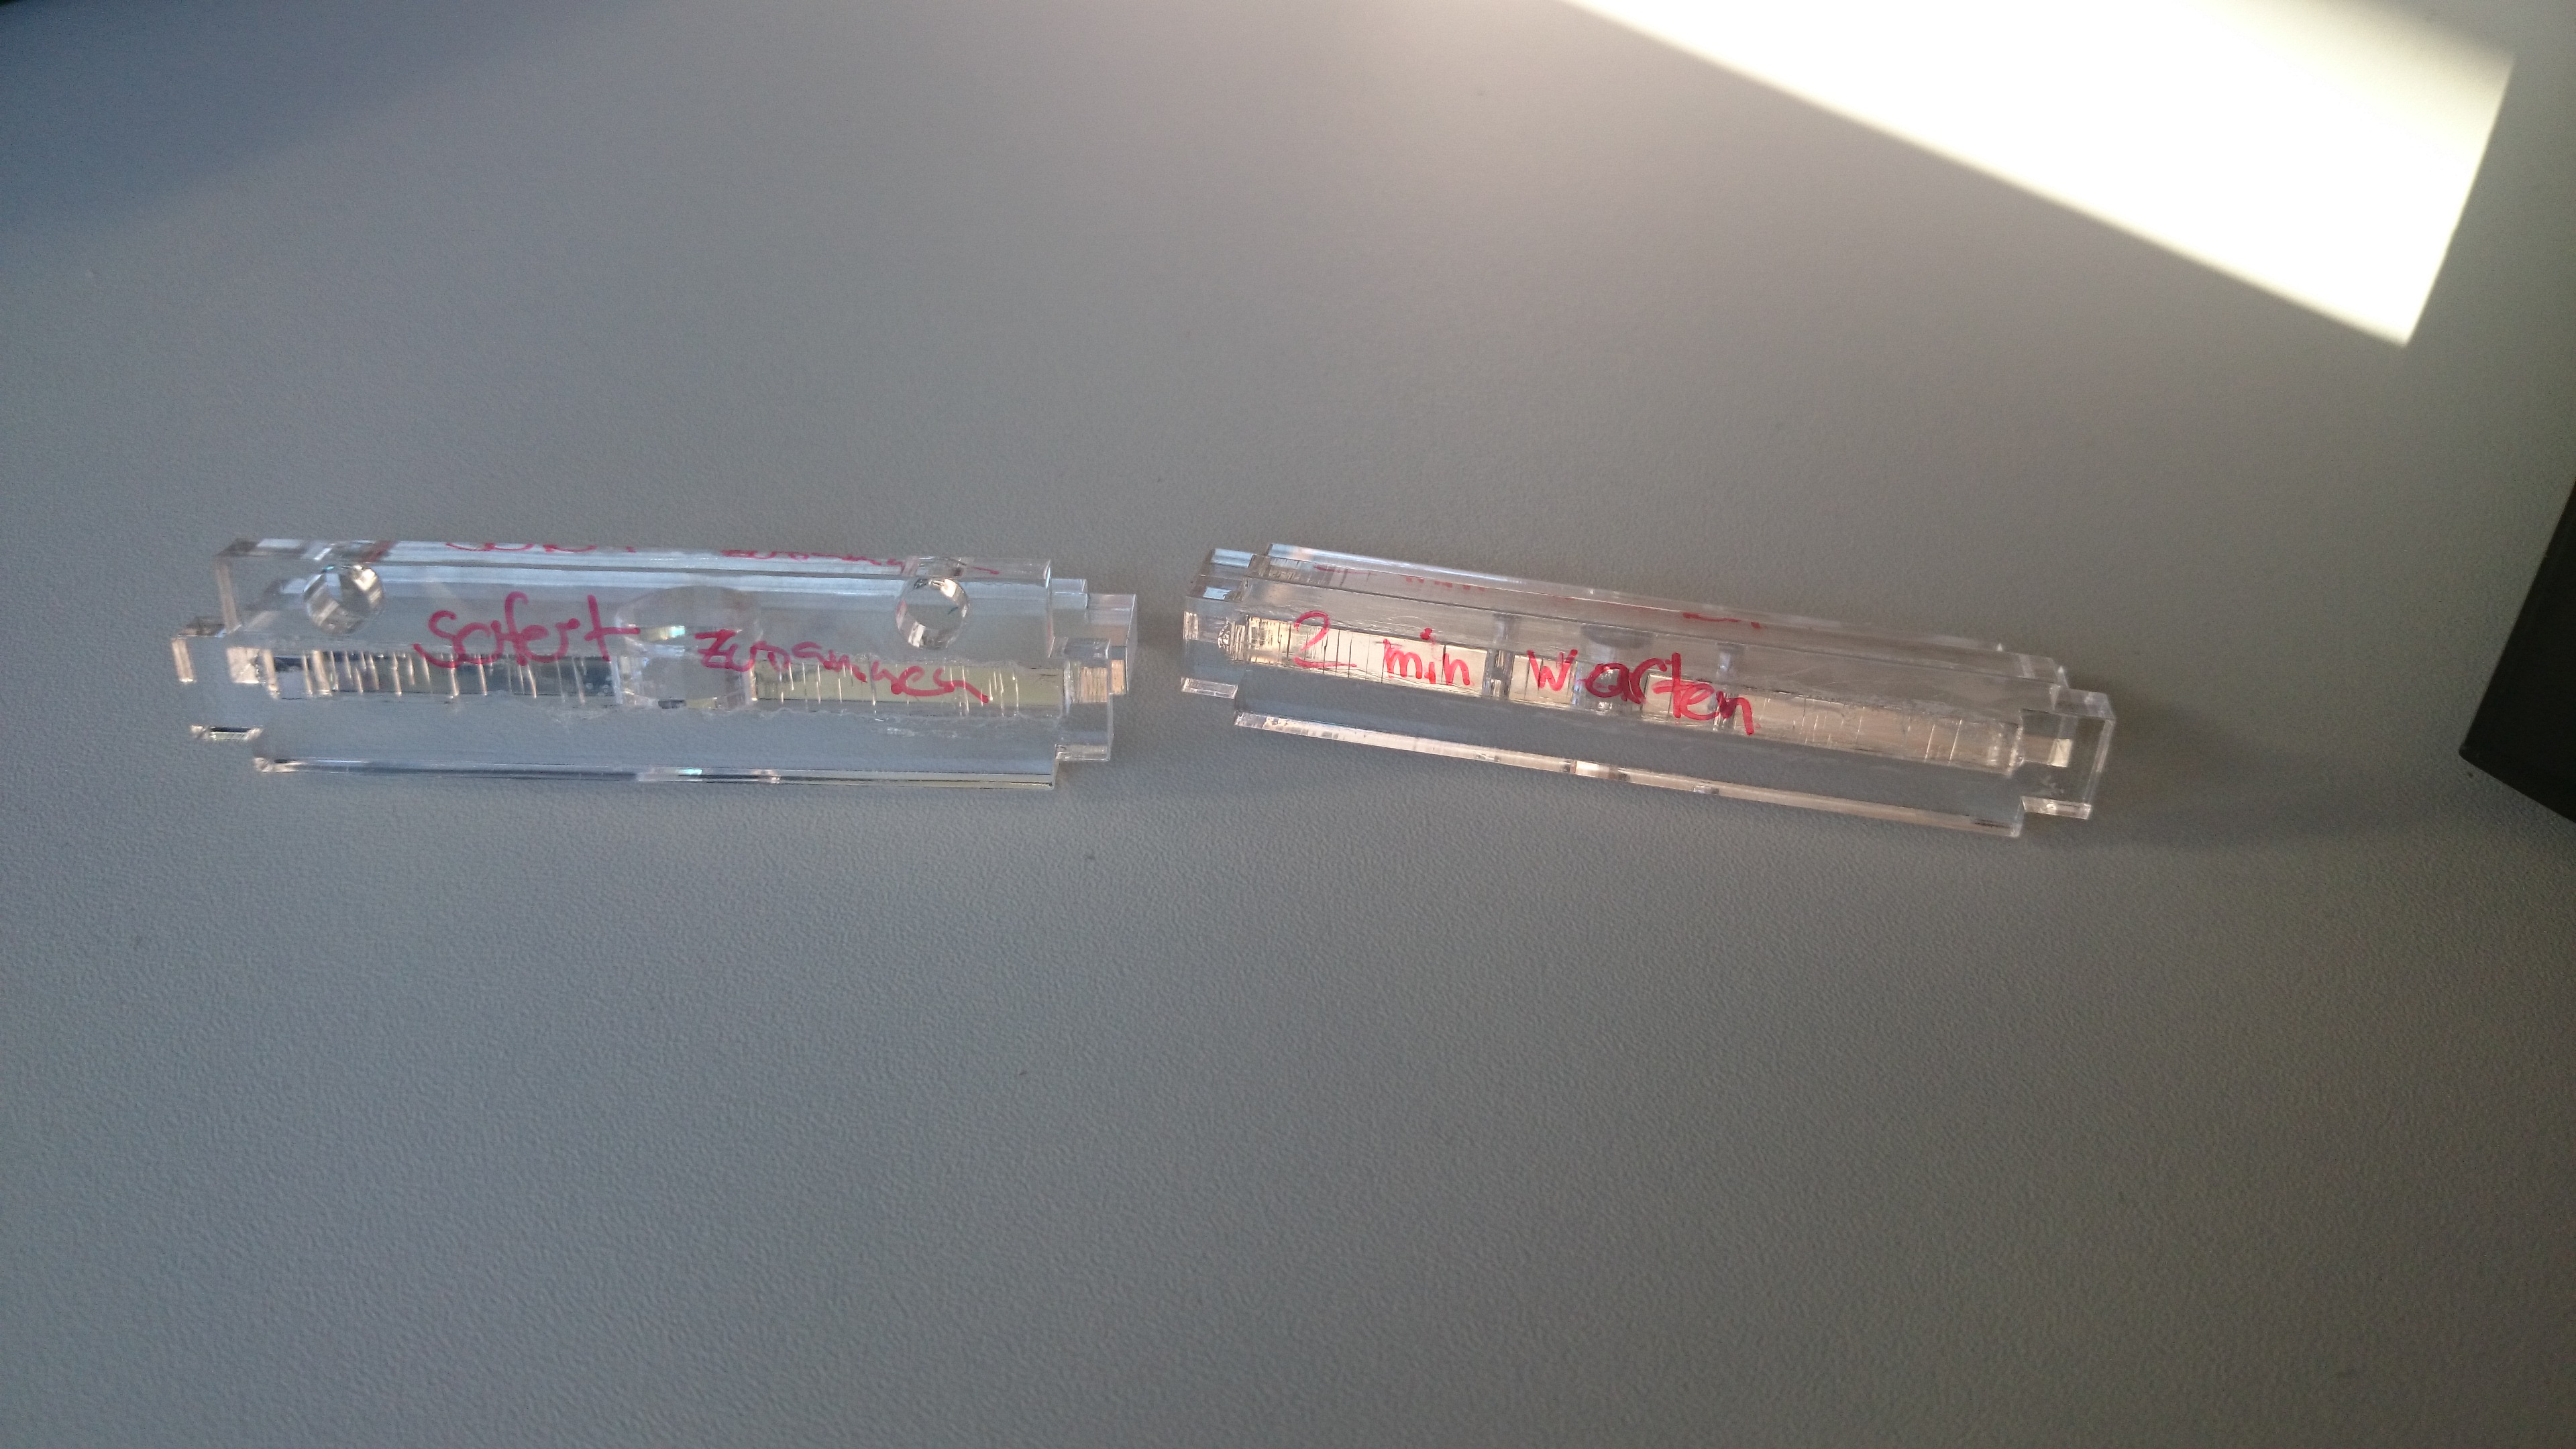
\includegraphics[width=0.7\textwidth,clip,trim=0cm 0cm 0cm 0cm]
	{Testberichte/Klebeversuch.jpg}
	\centering
	\caption{Klebeversuch mit UHU Kleber} 
	\label{abb:Klebeversuch}
\end{figure}
    
\end{docu}